\section{Equivalence Relations}

In general, we use the symbol $\equiv$ to denote equivalence relations, mostly between states of an automata. In general, we have automata $\mathcal{A}$ and $\mathcal{B}$ with states $p$ and $q$ from there respective state spaces. Our relations are then defined on $(\mathcal{A}, p) \equiv (\mathcal{B}, q)$.

\begin{defn}
	Assuming that $\mathcal{A}$ is a fixed automaton that is obvious in context and $p$ and $q$ are both states in $\mathcal{A}$, we shorten $(\mathcal{A}, p) \equiv (\mathcal{A}, q)$ to $p \equiv q$.
	
	Furthermore, we write $\mathcal{A} \equiv \mathcal{B}$ if for every $p$ in $\mathcal{A}$ there is a $q$ in $\mathcal{B}$ such that $(\mathcal{A}, p) \equiv (\mathcal{B}, q)$; and the same holds with $\mathcal{A}$ and $\mathcal{B}$ exchanged.
\end{defn}

\begin{defn}
	Let $\mathcal{A} = (Q_1, \Sigma, \delta_1)$ and $\mathcal{B} = (Q_2, \Sigma, \delta_2)$ be deterministic transition structures and let $\sim$ be an equivalence relation. We call $\sim$ a \emph{congruence relation} if for all $(\mathcal{A}, p) \sim (\mathcal{B}, q)$ and all $a \in \Sigma$, also $(\mathcal{A}, \delta_1(p, a)) \sim (\mathcal{B}, \delta_2(q, a))$.
\end{defn}

\begin{defn}
	Let $\sim$ be an equivalence relation. We define the \emph{congruence refinement} of $\sim$ as $\approx$ with $(\mathcal{A}, p) \approx (\mathcal{B}, q)$ iff for all $w \in \Sigma^*$, $(\mathcal{A}, \delta_1^*(p, w)) \sim (\mathcal{B}, \delta_2(q, w))$.
\end{defn}

\begin{lem}
	For a given equivalence relation $\sim$, the congruence refinement of $\sim$ is a congruence relation.
\end{lem}

\begin{proof}
	Assume towards a contradiction that there are $(\mathcal{A}, p) \approx (\mathcal{B}, q)$ such that $(\mathcal{A}, \delta_1(p, a)) \not\approx (\mathcal{B}, \delta_2(q, a))$. Thus, there is a $w \in \Sigma^*$ with $(\mathcal{A}, \delta_1^*(\delta_1(p, a), w)) \not\sim (\mathcal{B}, \delta_2(\delta_2(q, a), w))$. This means $(\mathcal{A}, \delta_1^*(p, aw)) \not\sim (\mathcal{B}, \delta_2(q, aw))$ and therefore $(\mathcal{A}, p) \not\approx (\mathcal{B}, q)$.
\end{proof}

\begin{lem}
	For a given equivalence relation $\sim$, the congruence refinement on a single automaton $\mathcal{A}$ can be computed in $\mathcal{O}(|\mathcal{A}| \cdot \log |\mathcal{A}|)$.
	\label{lem:general:congref_in_nlogn}
\end{lem}

\begin{proof}
	We refer to \cite{Hopcroft1971}, which describes a special case where $p \sim q$ iff $c(p) = c(q)$.
\end{proof}


\vspace{15pt}
The following is a comprehensive list of all relevant equivalence relations that we use.

\begin{itemize}
	\item Language equivalence, $\equiv_L$. Defined below.
	\item Moore equivalence, $\equiv_M$. Defined below.
	\item Priority almost equivalence, $\equiv_\text{\Ankh}$. Defined below.
	\item Delayed simulation equivalence, $\equiv_\text{de}$. Defined in section \ref{sect:fritzwilke}.
	\item Delayed simulation equivalence with resets, $\equiv_\text{deR}$. Defined in section \ref{sect:fritzwilke}.
	\item Iterated Moore equivalence, $\equiv_\text{IM}$. Defined in section \ref{sect:imoore}.
	\item Path refinement equivalence, $\equiv_\text{PR}$. Defined in section \ref{sect:pr}.
	\item Threshold Moore equivalence, $\equiv_\text{TM}^\sim$. Defined in section \ref{sect:tm}.
	\item Labeled SCC filter equivalence, $\equiv_\text{LSF}^{k,\sim}$. Defined in section \ref{sect:lsf}.
\end{itemize}

Immediately we define the three first of these relations and show that they are computable.

\vspace{5pt}

\subsection{Language Equivalence}

\begin{defn}
	Let $\mathcal{A}$ and $\mathcal{B}$ be $\omega$-automata. We define \emph{language equivalence} as $(\mathcal{A}, p) \equiv_L (\mathcal{B}, q)$ if and only if for all words $\alpha \in \Sigma^\omega$, $\mathcal{A}$ accepts $\alpha$ from $p$ iff $\mathcal{B}$ accepts $\alpha$ from $q$.
\end{defn}

\begin{lem}
	$\equiv_L$ is a congruence relation.
	\label{lem:general:L_congruence}
\end{lem}

\begin{proof}
	It is obvious that $\equiv_L$ is an equivalence relation. For two states $(\mathcal{A}, p) \equiv_L (\mathcal{B}, q)$ and some successors $p' = \delta_1(p, a)$ and $q' = \delta_2(q, a)$, it must be true that $(\mathcal{A}, p') \equiv_L (\mathcal{B}, q')$. Otherwise there is a word $\alpha \in \Sigma^\omega$ that is accepted from $p'$ and rejected from $q'$ (or vice-versa). Then $a \cdot \alpha$ is rejected from $p$ and accepted from $q$ and thus $p \not\equiv_L q$.
\end{proof}

\begin{lem}
	Language equivalence of a given DPA can be computed in $\mathcal{O}(|Q|^2 \cdot |c(Q)|^2)$.
\end{lem}

\begin{proof}
	The algorithm is based partially on \cite{HenzingerTelle1996}.
	
	Let $\mathcal{A} = (Q, \Sigma, \delta, c)$ be the DPA that we want to compute $\equiv_L$ on. We construct a labeled deterministic transition structure $\mathcal{B} = (Q \times Q, \Sigma, \delta', d)$ with $\delta'((p_1, p_2), a) = (\delta(p_1, a), \delta(p_2, a))$ and $d((p_1, p_2)) = (c(p_1), c(p_2)) \in \mathbb{N}^2$. Then, for every $i, j \in c(Q)$, let $\mathcal{B}_{i,j} = \mathcal{B} \upharpoonright_{Q_{i,j}}$ with $Q_{i,j} = \{ (p_1, p_2) \in Q \times Q \mid c(p_1) \geq i, c(p_2) \geq j \}$, i.e. remove all states which have first priority less than $i$ or second priority less than $j$.
	
	For each $i$ and $j$, let $S_{i,j} \subseteq 2^{Q \times Q}$ be the set of all SCCs in $\mathcal{B}_{i,j}$ and let $S = \bigcup_{i,j} S_{i,j}$. From this set $S$, remove all SCCs $s \subseteq Q \times Q$ in which the parity of the smallest priority in the first component differs from the parity of the smallest priority in the second component. The \enquote{filtered} set we call $S'$. For any two states $p, q \in Q$, $p \not\equiv_L q$ iff there is a pair $(p', q') \in \bigcup S'$ that is reachable from $(p, q)$ in $\mathcal{B}$.
	
	We omit the correctness proof of the algorithm here. Regarding the runtime, observe that $\mathcal{B}$ has size $\mathcal{O}(|Q|^2)$ and we create $\mathcal{O}(|c(Q)|^2)$ copies of it. All other steps like computing the SCCs can then be done in linear time in the size of the automata, which brings the total to $\mathcal{O}(|Q|^2 \cdot |c(Q)|^2)$.
\end{proof}

\vspace{5pt}

\subsection{Priority Almost Equivalence}

\begin{defn}
	Let $\mathcal{A} = (Q_1, \Sigma, \delta_1, c_1)$ and $\mathcal{B} = (Q_2, \Sigma, \delta_2, c_2)$ be DPAs. We define \emph{priority almost equivalence} as $(\mathcal{A}, p) \equiv_\text{\Ankh} (\mathcal{B}, q)$ if and only if for all words $\alpha \in \Sigma^\omega$, $c_1^*(p, \alpha)$ and $c_2^*(q, \alpha)$ differ at only finitely many positions.
\end{defn}

\begin{lem}
	Priority almost equivalence is a congruence relation.
	\label{lem:general:Ankh_congruence}
\end{lem}

\begin{proof} 
	It is obvious that $\equiv_\text{\Ankh}$ is an equivalence relation. For two states $(\mathcal{A}, p) \equiv_\text{\Ankh} (\mathcal{B}, q)$ and some successors $p' = \delta(p, a)$ and $q' = \delta(q, a)$, it must be true that $(\mathcal{A}, p') \equiv_\text{\Ankh} (\mathcal{B}, q')$. Otherwise there is a word $\alpha \in \Sigma^\omega$ such that $c_1^*(p', \alpha)$ and $c_2^*(q', \alpha)$ differ at infinitely many positions. Then $c_1^*(p, a \alpha)$ and $c_2^*(q, a \alpha)$ also differ at infinitely many positions and thus $(\mathcal{A}, p) \not\equiv_\text{\Ankh} (\mathcal{B}, q)$.
\end{proof}

The following definition is used as an intermediate step on the way to computing $\equiv_\text{\Ankh}$.

\begin{defn}
	Let $\mathcal{A} = (Q_1, \Sigma, \delta_1, c_1)$ and $\mathcal{B} = (Q_2, \Sigma, \delta_2, c_2)$ be DPAs. We define the deterministic Büchi automaton $\mathcal{A} \intercal \mathcal{B} = (Q_1 \times Q_2, \Sigma, \delta_\intercal, F_\intercal)$ with $\delta_\intercal((q_1, q_2), a) = (\delta_1(q_1, a), \delta_2(q_2, a))$. The transition structure is a common product automaton.
	
	The final states are $F_\intercal = \{ (p, q) \in Q_1 \times Q_2 \mid c_1(p) \neq c_2(q) \}$, i.e. every pair of states at which the priorities differ. 
\end{defn}

\begin{lem}
	$\mathcal{A} \intercal \mathcal{B}$ can be computed in time $\mathcal{O}(|Q_1| \cdot |Q_2|)$.
	\label{lem:general:intercal_runtime}
\end{lem}

\begin{proof}
	The definition already provides a rather straightforward description of how to compute $\mathcal{A} \intercal \mathcal{B}$. Each state only requires constant time (assuming that $\delta$ and $c$ can be evaluated in such) and has $|\mathcal{A}| \cdot |\mathcal{B}|$ many states.
\end{proof}

\begin{lem}
	Let $\mathcal{A} = (Q_1, \Sigma, \delta_1, c_1)$ and $\mathcal{B} = (Q_2, \Sigma, \delta_2, c_2)$ be DPAs. $(\mathcal{A}, p) \equiv_\text{\Ankh} (\mathcal{B}, q)$ iff $L(\mathcal{A} \intercal \mathcal{B}, (p, q)) = \emptyset$. 
	\label{lem:general:intercal_prioalmostequiv}
\end{lem}

\begin{proof}
	For the first direction of implication, let $L(\mathcal{A} \intercal \mathcal{B}, (p_0, q_0)) \neq \emptyset$, so there is a word $\alpha$ accepted by that automaton. Let $(p, q) (p_1, q_1) (p_2, q_2) \cdots$ be the accepting run on $\alpha$. Then $p p_1 \cdots$ and $q q_1 \cdots$ are the runs of $\mathcal{A}$ and $\mathcal{B}$ on $\alpha$ respectively. Whenever $(p_i, q_i) \in F_\intercal$, $p_i$ and $q_i$ have different priorities. As the run of the product automaton vists infinitely many accepting states, $\alpha$ is a witness for $p$ and $q$ being not priority almost-equivalent.
	
	For the second direction, let $p$ and $q$ be not priority almost-equivalent, so there is a witness $\alpha$ at which infinitely many positions differ in priority. Analogously to the first direction, this means that the run of $\mathcal{A} \intercal \mathcal{B}$ on the same word is accepting and therefore the language is not empty.
\end{proof}

\begin{cor}
	Priority almost equivalence of a given DPA can be computed in quadratic time.
\end{cor}

\begin{proof}
	By Lemma \ref{lem:general:intercal_runtime}, we can compute $\mathcal{A} \intercal \mathcal{A}$ in quadratic time. The emptiness problem for deterministic B\"uchi automata is solvable in linear time by checking reachability of loops that contain a state in $F$. 
\end{proof}

\vspace{5pt}

\subsection{Moore Equivalence}

\begin{defn}
	Let $\mathcal{A} = (Q_1, \Sigma, \delta_1, c_1)$ and $\mathcal{B} = (Q_2, \Sigma, \delta_2, c_2)$ be DPAs. We define \emph{Moore equivalence} as $(\mathcal{A}, p) \equiv_M (\mathcal{B}, q)$ if and only if for all words $w \in \Sigma^*$, $c_1(\delta^*(p, w)) = c_2(\delta^*(q, w))$.
\end{defn}

\begin{lem}
	Moore equivalence is the congruence refinement of $\sim$ with $(\mathcal{A}, p) \sim (\mathcal{B}, q)$ iff $c(p) = c(q)$.
\end{lem}

\begin{cor}
	$\equiv_M$ is a congruence relation.
	\label{cor:general:M_congruence}
\end{cor}

\begin{cor}
	Moore equivalence of a given DPA can be computed in log-linear time.
	\label{cor:general:M_loglin}
\end{cor}



\vspace{10pt}

\begin{theorem}
	$\equiv_M \,\subseteq\, \equiv_\text{\Ankh} \,\subseteq\, \equiv_L$
	\label{thm:general:M_subs_Ankh_subs_L}
\end{theorem}

\begin{proof}
	Let $\mathcal{A} = (Q_1, \Sigma, \delta_1, c_1)$ and $\mathcal{B} = (Q_2, \Sigma, \delta_2, c_2)$ be DPAs with states $q_1 \in Q_1$ and $q_2 \in Q_2$. 
	
	At first, let $(\mathcal{A}, q_1) \equiv_M (\mathcal{B}, q_2)$ and assume towards a contradiction that $(\mathcal{A}, q_1) \not\equiv_\text{\Ankh} (\mathcal{B}, q_2)$, so there is a word $\alpha \in \Sigma^\omega$ such that $c_1^*(q_1, \alpha)$ and $c_2^*(q_2, \alpha)$ differ at infinitely many positions. In particular, there is some $w \sqsubseteq \alpha$ such that $c_1(\delta_1^*(q_1, w)) \neq c_2(\delta_2^*(q_2, w))$. This would be a contradiction to $(\mathcal{A}, q_1) \equiv_M (\mathcal{B}, q_2)$.
	
	Now assume that $(\mathcal{A}, q_1) \equiv_\text{\Ankh} (\mathcal{B}, q_2)$ and let $\alpha \in \Sigma^\omega$. Let $\rho_1$ and $\rho_2$ be the runs of $\mathcal{A}$ and $\mathcal{B}$ on $\alpha$ starting in $q_1$ and $q_2$. Because $(\mathcal{A}, q_1) \equiv_\text{\Ankh} (\mathcal{B}, q_2)$ is true, there is a position $n$ such that $c_1(\rho_1[n,\omega]) = c_2(\rho_2[n,\omega])$ and therefore $\text{Inf}(c_1(\rho_1[n,\omega])) = \text{Inf}(c_2(\rho_2[n,\omega]))$, which means that the runs have the same acceptance. Thus, $(\mathcal{A}, q_1) \equiv_L (\mathcal{B}, q_2)$.
\end{proof}






\section{Representative Merge}

\begin{defn}
	Let $\mathcal{A} = (Q, \Sigma, \delta, c)$ be a DPA and let $\emptyset \neq C \subseteq M \subseteq Q$. Let $\mathcal{A}' = (Q', \Sigma, \delta', c')$ be another DPA. We call $\mathcal{A}'$ a \emph{representative merge of $\mathcal{A}$ w.r.t. $M$ by candidates $C$} if it satisfies the following:
	\begin{itemize}
		\item There is a state $r_M \in C$ such that $Q' = (Q \setminus M) \cup \{r_M\}$.
		\item $c' = c\upharpoonright_{Q'}$.
		\item Let $p \in Q'$ and $\delta(p, a) = q$. If $q \in M $, then $\delta'(p, a) = r_M$. Otherwise, $\delta'(p, a) = q$. 
	\end{itemize}
	
	We call $r_M$ the \emph{representative} of $M$ in the merge. We might omit $C$ and implicitly assume $C = M$.
\end{defn}

\begin{defn}
	Let $\mathcal{A} = (Q, \Sigma, \delta, c)$ be a DPA and let $\mu : D \rightarrow (2^\mathcal{Q} \setminus \emptyset)$ be a function for some $D \subseteq 2^Q$. We call $\mu$ a \emph{merger function} if 
	\begin{itemize}
		\item all sets in $D$ are pairwise disjoint; and
		\item for $U = \bigcup D$ and all sets $X \in D$, $\mu(X) \cap (U \setminus X) = \emptyset$
	\end{itemize}
	
	A DPA $\mathcal{A}'$ is a representative merge of $\mathcal{A}$ w.r.t. $\mu$ if there is an enumeration $X_1, \dots, X_{|D|}$ of $D$ and a sequence of automata $\mathcal{A}_0, \dots, \mathcal{A}_{|D|}$ such that $\mathcal{A}_0 = \mathcal{A}$, $\mathcal{A}_{|D|} = \mathcal{A}'$ and every $\mathcal{A}_{i+1}$ is a representative merge of $\mathcal{A}_i$ w.r.t. $X_{i+1}$ by candidates $\mu(X_{i+1})$.
\end{defn}

\vspace{5pt}

The following Lemma formally proofs that this definition actually makes sense, as building representative merges is commutative if the merge sets are disjoint.

\begin{lem}
	Let $\mathcal{A} = (Q, \Sigma, \delta, c)$ be a DPA and let $M_1, M_2 \subseteq Q$. Let $\mathcal{A}_1$ be a representative merge of $\mathcal{A}$ w.r.t. $M_1$ by some candidates $C_1$. Let $\mathcal{A}_{12}$ be a representative merge of $\mathcal{A}_1$ w.r.t. $M_2$ by some candidates $C_2$. If $M_1$ and $M_2$ are disjoint, then there is a representative merge $\mathcal{A}_2$ of $\mathcal{A}$ w.r.t. $M_2$ by candidates $C_2$ such that $\mathcal{A}_{12}$ is a representative merge of $\mathcal{A}_2$ w.r.t $M_1$ by candidates $C_1$.
\end{lem}

\begin{proof}
	By choosing the same representative $r_{M_1}$ and $r_{M_2}$ in the merges, this is a simple application of the definition.
\end{proof}


\vspace{10pt}

The following Lemma, while simple to prove, is interesting and will find use in multiple proofs of correctness later on.

\begin{lem}
	Let $\mathcal{A}$ be a DPA. Let $\sim$ be a congruence relation on $Q$ and let $M \subseteq Q$ such that for all $x, y \in M$, $x \sim y$. Let $\mathcal{A}'$ be a representative merge of $\mathcal{A}$ w.r.t. $M$ by candidates $C$. Let $\rho$ and $\rho'$ be runs of $\mathcal{A}$ and $\mathcal{A}'$ on some $\alpha$. Then for all $i$, $(\mathcal{A}, \rho(i)) \sim (\mathcal{A}, \rho'(i))$.
	\label{lem:general:cong_stays_in_merge}
\end{lem}

\begin{proof}
	We use a proof by induction. For $i = 0$, we have $\rho(0) = q_0$ for some $q_0 \in Q$ and $\rho'(0) = r_{[q_0]_M}$. By choice of the representative, $q_0 \in M$ and $r_{[q_0]_M} \in M$ and thus $q_0 \sim r_{[q_0]_M}$.
	
	Now consider some $i+1 > 0$. Then $\rho'(i+1) = r_{[q]_M}$ for $q = \delta(\rho'(i), \alpha(i))$. By induction we know that $\rho(i) \sim \rho'(i)$ and thus $\delta(\rho(i), \alpha(i)) = \rho(i+1) \sim q$. Further, we know $q \sim r_{[q]_M}$ by the same argument as before. Together this lets us conclude in $\rho(i+1) \sim q \sim \rho'(i+1)$.
\end{proof}

\vspace{10pt}

The following is a comprehensive list of all relevant merger functions that we use.

\begin{itemize}
	\item Quotient merger, $\mu_\div^\sim$. Defined below.
	\item Moore merger, $\mu_M$. Defined below.
	\item Skip merger, $\mu_\text{skip}^\sim$. Defined in section \ref{sect:skipper}.
	\item Delayed simulation merger, $\mu_\text{de}$. Defined in section \ref{sect:fritzwilke}.
	\item Path refinement merger, $\mu_\text{PR}^\lambda$. Defined in section \ref{sect:pr}.
	\item Treshold Moore merger, $\mu_\text{TM}^\sim$. Defined in section \ref{sect:tm}.
	\item Labeled SCC Filter merger, $\mu_\text{LSF}^{k,\sim}$. Defined in section \ref{sect:lsf}.
\end{itemize}

\vspace{5pt}

\subsection{Quotient merger}
\begin{defn}
	Let $\sim$ be a congruence relation. We define the \emph{quotient merger} $\mu^\sim_\div : \mathfrak{C}(\sim) \rightarrow 2^Q, \kappa \mapsto \kappa$. 
\end{defn}


\begin{lem}
\label{lem:general:congrel_prio_implies_moore}
	Let $\mathcal{A} = (Q, \Sigma, \delta, c)$ be a DPA and let $\sim$ be a congruence relation such that $p \sim q$ implies $c(p) = c(q)$. Then $\mathcal{A}$ is Moore equivalent to every representative merge w.r.t. $\mu_\div^\sim$.
\end{lem} 

\begin{proof} 
	Let $\mathcal{A}' = (Q', \Sigma, \delta', c')$ be a representative merge. For every $q \in Q$, we prove that $(\mathcal{A}, q) \equiv_M (\mathcal{A}', r_{[q]_\sim})$. Since all states in $\mathcal{A}'$ are representatives of that form and every representative exists in $\mathcal{A}$ as well, this suffices to prove Moore equivalence.
	
	Let $\alpha \in \Sigma^\omega$ be a word and let $\rho$ and $\rho'$ be the runs of $\mathcal{A}$ and $\mathcal{A}'$ on $\alpha$ starting in $q$ and $r_{[q]_\sim}$. For every $i \in \mathbb{N}$, we have $\rho'(i) = [\rho(i)]_\sim$ and thus $c'(\rho'(i)) = c(\rho(i))$. Therefore, $\rho$ is accepting iff $\rho'$ is accepting.
\end{proof}



\subsection{Moore merger}
\begin{defn}
	We define the special \emph{Moore merger} $\mu_M = \mu_\div^{\equiv_M}$.
\end{defn}

\begin{lem}
	Let $\mathcal{A}$ be a DPA and let $\mathcal{A}'$ be a representative merge of $\mathcal{A}$ w.r.t. $\mu_M$. Then $\mathcal{A} \equiv_L \mathcal{A}'$.
\end{lem}

\begin{proof}
	Directly implied by Lemma \ref{lem:general:congrel_prio_implies_moore} and Theorem \ref{thm:general:M_subs_Ankh_subs_L}.
\end{proof}

\vspace{5pt}

In figure \ref{fig:general:empirical_moore_size_hist}, the efficiency of $\mu_M$ on different types of automata is shown. On the \textsf{gendet} and \textsf{detnbaut} classes, barely any state reduction is achieved. \textsf{gendet} lacks patterns in its automata and \textsf{detnbaut} already has certain minimization techniques applied during generation. \textsf{detspot} on the other hand shows some small but noticeable reduction. In figure \ref{fig:general:empirical_moore_reduct_abs}, we can see that the number of removed states is roughly proportional to the number of total states, which is no big surprise.

As is to be expected from Corollary \ref{cor:general:M_loglin} and confirmed in figure \ref{fig:skip:empirical_moore_time}, the Moore merger is very easy to compute.


\begin{figure}
	\centering
	\begin{minipage}{0.49\textwidth}
		\includegraphics[page=6,height=.3\textheight]{../data/analysis/hopcroft/gendet_ap1.pdf} 
		\includegraphics[page=6,height=.3\textheight]{../data/analysis/hopcroft/detspot_ap1.pdf} 
		\includegraphics[page=6,height=.3\textheight]{../data/analysis/hopcroft/detnbaut_ap1.pdf} 
		\caption{Relative state reduction of different automata using $\mu_M$.}
		\label{fig:general:empirical_moore_size_hist}
	\end{minipage}
	\hfill
	\begin{minipage}{0.49\textwidth}
		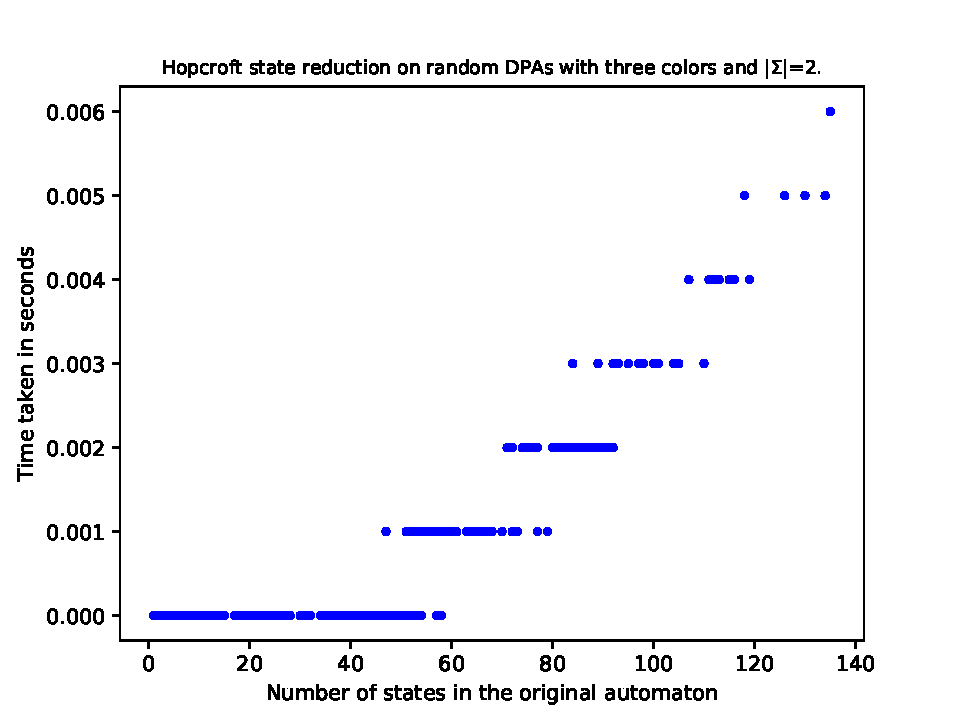
\includegraphics[page=1,height=.3\textheight]{../data/analysis/hopcroft/gendet_ap1.pdf} 
		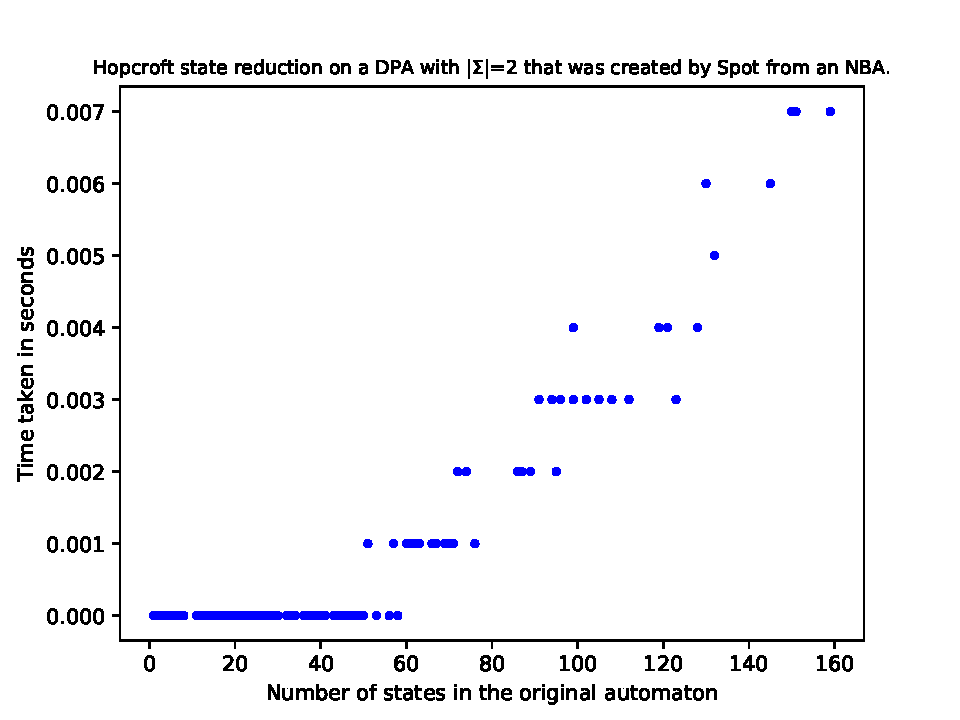
\includegraphics[page=1,height=.3\textheight]{../data/analysis/hopcroft/detspot_ap1.pdf} 
		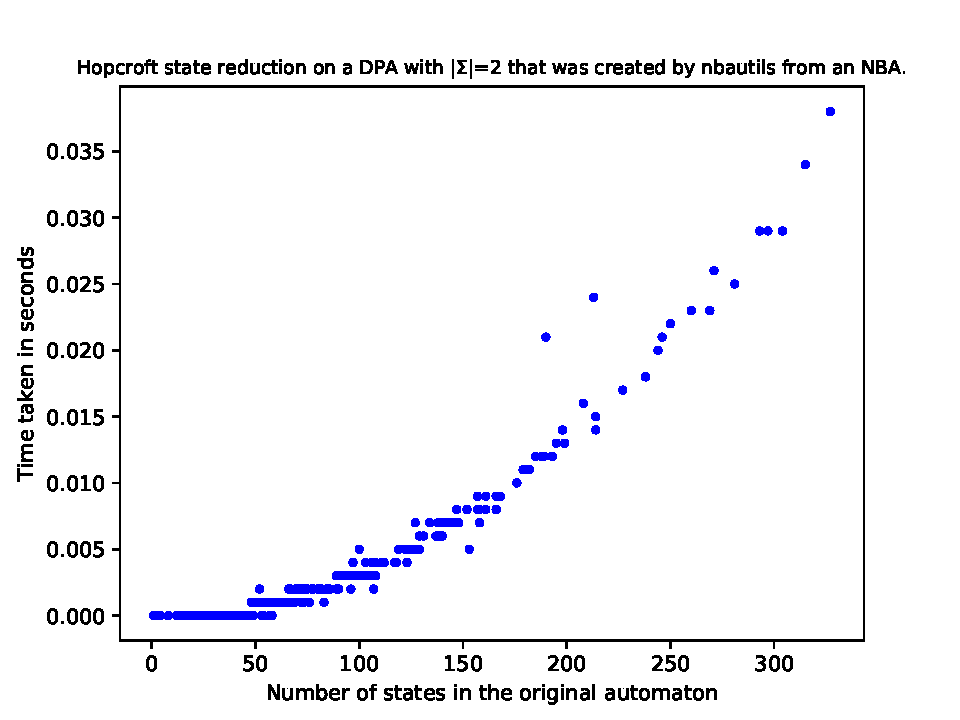
\includegraphics[page=1,height=.3\textheight]{../data/analysis/hopcroft/detnbaut_ap1.pdf} 
		\caption{Time of the relative state reduction of different automata using $\mu_M$.}
		\label{fig:skip:empirical_moore_time}
	\end{minipage}
\end{figure}

\begin{figure}
	\centering
	\includegraphics[page=2,height=.4\textheight]{../data/analysis/hopcroft/detspot_ap1.pdf} 
	\caption{Relative state reduction of \textsf{detspot} automata using $\mu_M$.}
	\label{fig:general:empirical_moore_reduct_abs}
\end{figure}



\vspace{5pt}





\section{Reachability}

\begin{defn}
	Let $\mathcal{S} = (Q, \Sigma, \delta)$ be a deterministic transition structure. We define the \emph{reachability order} $\preceq_\text{reach}^\mathcal{S}$ as $p \preceq_\text{reach}^\mathcal{S} q$ if and only if $q$ is reachable from $p$. 
\end{defn}

We want to note here that we always assume for all automata to only have one connected component, i.e. for all states $p$ and $q$, there is a state $r$ such that $p$ and $q$ are both reachable from $r$. In practice, most automata have an predefined initial state and a simple depth first search can be used to eliminate all unreachable states.

\begin{lem}
	$\preceq_\text{reach}^\mathcal{S}$ is a preorder.
\end{lem}

\begin{defn}
	Let $\mathcal{S} = (Q, \Sigma, \delta)$ be a deterministic transition structure. We call a relation $\preceq$ a \emph{total extension of reachability} if it is a minimal superset of $\preceq_\text{reach}^\mathcal{S}$ that is also a total preorder.
	
	For $p \preceq q$ and $q \preceq p$, we write $p \simeq q$.
\end{defn}

\begin{lem}
	For a given deterministic transition structure $\mathcal{S}$, a total extension of reachability is computable in $\mathcal{O}(|\mathcal{S}|)$.
	\label{lem:general:reach_topo_lintime}
\end{lem}

\begin{proof}
	Using e.g. Kosaraju's algorithm \cite{Sharir81}, the SCCs of $\mathcal{A}$ can be computed in linear time. We can now build a DAG from $\mathcal{A}$ by merging all states in an SCC into a single state; iterate over all transitions $(p, a, q)$ and add an $a$-transition from the merged representative of $p$ to that of $q$. Assuming efficient data structures for the computed SCCs, this DAG can be computed in $O(|\mathcal{A}|)$ time.
	
	To finish the computation of $\preceq$, we look for a topological order on that DAG. This is a total preorder on the SCCs that is compatible with reachability. All that is left to be done is to extend that order to all states.
\end{proof}




\section{Changing Priorities}
As we mentioned earlier, state reduction of DPAs is difficult and minimization is an NP-hard problem. Priorities of states on the other hand are generally easier to modify. A few of these possibilities are considered in this section.

\begin{lem}
\label{lem:general:trivial_scc_dont_matter}
	Let $\mathcal{A} = (Q, \Sigma, \delta, c)$ be a DPA and let $\{s\} \subseteq Q$ be a trivial SCC in $\mathcal{A}$. Let $\mathcal{A}' = (Q, \Sigma, \delta, c')$ be a copy of $\mathcal{A}$ with the only exception that $c'(s) = k$ for some arbitrary $k$. Then $\mathcal{A} \equiv_L \mathcal{A}'$.
\end{lem}

\begin{proof}
	Let $q \in Q$ be any state. We show that $L(\mathcal{A}, q) = L(\mathcal{A}', q)$. Let $\rho$ and $\rho'$ be the runs of $\mathcal{A}$ and $\mathcal{A}'$ starting in $q$ on some $\alpha \in \Sigma^\omega$. As $s$ lies in a trivial SCC, the runs visit that state at most once. Therefore, $\text{Inf} c(\rho) = \text{Inf} c'(\rho')$ and the runs have the same acceptance.
\end{proof}

\vspace{10pt}

An interesting property that parity automata can have is being \emph{normalized}. Even more important is that a normalized version of a DPA can be computed rather easily.

\begin{defn}
	Let $\mathcal{A} = (Q, \Sigma, \delta, c)$ be a DPA. We call $\mathcal{A}$ \emph{$c$-normalized} if for every state $q \in Q$ that does not lie in a trivial SCC and all priorities $k \leq c(q)$, there is a path from $q$ to $q$ such that the lowest priority visited is $k$.
\end{defn}


Algorithm \ref{alg:general:normalize_c} shows how an equivalent normalized priority function can be computed in $\mathcal{O}(|Q| \cdot |c(Q)|)$. The algorithm is a slight adaption of that presented in \cite{CartonMaceiras99}, which is why we will not go into further details here and just refer to the original source.

\begin{algorithm}[h!]
  \caption{Normalizing the priority function of a DPA.}
  \label{alg:general:normalize_c}
  \begin{algorithmic}[1]
    \Function{Normalize}{$\mathcal{A}$}
      \State $c' : Q \rightarrow \mathbb{N}, q \mapsto c(q)$
      \State \Call{M}{$\mathcal{A}$, $c'$}
      \State \Return{$c'$}
    \EndFunction
    \Statex
    \Function{M}{$\mathcal{A} \upharpoonright_P$, $c'$}
      \If{$P = \emptyset$}
        \State \Return 0
      \EndIf
      \State $min \gets 0$
      \For{SCC $S$ in $\mathcal{A} \upharpoonright_P$}
        \State $m := \min c(S) \mod 2$
        \State $X := c^{-1}(m)$
        \For{$q \in X$}
          \State $c'(q) \gets m$
        \EndFor
        \State $S' := S \setminus X$
        \State $m' \gets $\Call{M}{$\mathcal{A} \upharpoonright_{S'}$, $c'$}
        \If{$m'$ even}
          \If{$m$ even}
            \State $\delta := m$
          \Else
            \State $\delta := m-2$
          \EndIf
        \Else
          \State $\delta := m-1$
        \EndIf
        \For{$q \in S'$}
          \State $c'(q) \gets c'(q) - \delta$
        \EndFor
        \State $min \gets \min \{min, m\}$
      \EndFor
      \State \Return{$min$}
    \EndFunction
  \end{algorithmic}
\end{algorithm}








